%% LaTeX-Beamer template for KIT design
%% by Erik Burger, Christian Hammer
%% title picture by Klaus Krogmann
%%
%% version 2.1
%%
%% mostly compatible to KIT corporate design v2.0
%% http://intranet.kit.edu/gestaltungsrichtlinien.php
%%
%% Problems, bugs and comments to
%% burger@kit.edu

\documentclass[18pt]{beamer}

%% SLIDE FORMAT

% use 'beamerthemekit' for standard 4:3 ratio
% for widescreen slides (16:9), use 'beamerthemekitwide'
\usepackage{listings}
\usepackage{templates/beamerthemekit}
\usepackage{algorithm}
\usepackage{algorithmic}

% \usepackage{templates/beamerthemekitwide}

%% TITLE PICTURE

% if a custom picture is to be used on the title page, copy it into the 'logos'
% directory, in the line below, replace 'mypicture' with the 
% filename (without extension) and uncomment the following line
% (picture proportions: 63 : 20 for standard, 169 : 40 for wide
% *.eps format if you use latex+dvips+ps2pdf, 
% *.jpg/*.png/*.pdf if you use pdflatex)

\titleimage{logologo}

%% TITLE LOGO

% for a custom logo on the front page, copy your file into the 'logos'
% directory, insert the filename in the line below and uncomment it

%\titlelogo{mylogo}

% (*.eps format if you use latex+dvips+ps2pdf,
% *.jpg/*.png/*.pdf if you use pdflatex)

%% TikZ INTEGRATION

% use these packages for PCM symbols and UML classes
% \usepackage{templates/tikzkit}
% \usepackage{templates/tikzuml}

% the presentation starts here

\title[Mathe 1]{Mathe 1}
%\subtitle{Something for XYZ 2009}
\author{Charlotte P., Lena W., Vera C., Christian K.}

\institute{ITI Wagner \& IPD Tichy}

% Bibliography

\usepackage[citestyle=authoryear,bibstyle=numeric,hyperref,backend=biber]{biblatex}
\addbibresource{templates/example.bib}
\bibhang1em

\begin{document}

% change the following line to "ngerman" for German style date and logos
\selectlanguage{ngerman}

%title page
\begin{frame}
\titlepage
\end{frame}

%table of contents
\begin{frame}{Gliederung}
\tableofcontents
\end{frame}

\section {Big Integer}
\begin{frame}{Big integer}
\begin {itemize}
\item die maximale Zahl ist gr"o"ser als integer?
 
\item nehme long long

\item die Zahl ist gr"o"ser als long long
 
\item ?????????????????????????????????? (Panik) 
\end {itemize}
\end{frame}

\begin{frame}{Big integer - Java nutzen}
\begin {itemize}
\item import java.math.BigInteger
\item Konstruktor: BigInteger(String val)
\item Methoden:
\begin {itemize}
\item BigInteger add(BigInteger val)
\item BigInteger multiply(BigInteger val)
\item BigInteger subtract(BigInteger val)
\item BigInteger abs()
\item BigInteger compareTo(BigInteger val)
\item BigInteger[]  divideAndRemainder(BigInteger val) (Division mit Rest)
\item BigInteger gcd(BigInteger val)
\end {itemize}
\end {itemize}
\end{frame}

\begin{frame} {C++? Selbst implementieren!}
Schriftliche Addition, Beispiel: \\
String $x$ = " 12035"  \\
String $y$ = " 389" \\
\pause
vector $v_{x}$ = (5,3,0,2,1)\\
vector $v_{y}$ = (9,8,3,0,0)\\
vector $v_{z}$ = ()\\
\pause
$v_{z} = (4)$, "Ubertrag = 1\\
\pause
$v_{z} = (4,2)$, "Ubertrag = 1\\
\pause
$v_{z} = (4,2,4)$, "Ubertrag = 0\\
\pause
$v_{z} = (4,2,4,2)$, "Ubertrag = 0\\
\pause
$v_{z} = (4,2,4,2,1)$, "Ubertrag = 0\\
In $v_{z}$ steht das gespiegelte Ergebnis der Addition
\end{frame} 
 
\begin{frame} {Karazuba-Multiplikation}
Beobachtung: $(a_{0}+a_{1})\cdot(b_{0}+b_{1})=a_{0}\cdot b_{0} + a_{1}\cdot b_{1} + a_{1}\cdot b_{0}+
a_{0}\cdot b_{1}$
\scalebox{1.0}{
\begin{minipage}{0.9\linewidth}
\begin{algorithm} [H]
\scriptsize 
\caption{recMult(int a, int b)}
\begin{algorithmic}
\REQUIRE $a$ und $b$ haben $n$ Ziffern, sei $k=\lfloor n/2 \rfloor$ 
\IF{$n = 1$}
\STATE return $a\cdot b$
\ENDIF
\STATE schreibe a als $a_{1} \cdot B^{k} + a_{0}$
\STATE schreibe b als $b_{1} \cdot B^{k} + b_{0}$
\STATE $c_{11}=recMult(a_{1}, b_{1})$
\STATE $c_{00}=recMult(a_{0}, b_{0})$
\STATE return $c_{11} \cdot B^{2k}+(recMult((a_{1}+a_{0}),(b_{1}+b_{0}))-c_{11}-c_{00})\cdot B^{k} + c_{00}$
\end{algorithmic}
\end{algorithm}
\end{minipage}
}
\end{frame}

\section {Exponentiation by squaring}
\begin{frame} {Naive Exponentiation}
\scalebox{1.0}{
\begin{minipage}{1.0\linewidth}
\begin{algorithm} [H]
\scriptsize 
\caption{Bereche $y = x^n$ naiv}
\begin{algorithmic}
 
\REQUIRE $n \geq 0 \vee x \neq 0$
\ENSURE $y = x^n$
\STATE $y \leftarrow 1$
\IF{$n < 0$}
\STATE $X \leftarrow 1 / x$
\STATE $N \leftarrow -n$
\ELSE
\STATE $X \leftarrow x$
\STATE $N \leftarrow n$
\ENDIF
\WHILE{$N \neq 0$}
\STATE $y \leftarrow y \cdot X$
\STATE $N \leftarrow N-1$
\ENDWHILE
\STATE return $y$
\end{algorithmic}
\end{algorithm}
\end{minipage}
}
Bei ICPC gehen wir davon aus, dass Multiplikation zweier Zahlen in $\mathcal{O}(1)$ liegt, also naive Exponentiation in $\mathcal{O}(n)$
\end{frame}

\begin{frame} {Idee}
Beobachtung:
\begin{equation}
   x^{n} =
   \begin{cases}
     (x^{2})^{n/2} & \text{f"ur n gerade} \\
      x\cdot(x^{2})^{(n-1)/2} & \text{f"ur n ungerade} \\
   \end{cases}
\end{equation}
\end{frame}

\begin{frame} {Exponentiation by Squaring, rekursiv}
\scalebox{1.0}{
\begin{minipage}{1.0\linewidth}
\begin{algorithm} [H]
\scriptsize 
\caption{Exponentiation(n, x) (rekursiv)}
\begin{algorithmic}
\IF{$n < 0$}
\STATE {return Exponentiation(-$n, 1/$x)}
\ELSIF {$n = 0$}
\STATE {return 1}
\ELSIF {$n = 1$} 
\STATE {return x}
\ELSIF {$n$ modulo $2 = 0$}
\STATE {return Exponentiation($n/2$, $x \cdot x$)}
\ELSE \STATE{return $x \cdot Exponentiation((n-1)/2, x \cdot x)$}
\ENDIF
\end{algorithmic}
\end{algorithm}
\end{minipage}
}
Da Multiplikation konstant viel Zeit ben"otigt, liegt die Exponentiation in $\mathcal{O}(log(n))$
\end{frame}

\begin{frame} {Beispiel}
$2^ {10638} = (2^{5319})^{2}  $ \\
$2^ {5319} = 2 \cdot (2^{2659})^{2}  $ \\
$2^ {2659} = 2 \cdot (2^{1329})^{2}  $ \\
$2^ {1329} = 2 \cdot (2^{664})^{2}  $ \\
$2^ {664} = (2^{332})^{2}  $ \\
$2^ {332} = (2^{166})^{2}  $ \\
$2^ {166} = (2^{83})^{2}  $ \\
$2^ {83} = 2 \cdot (2^{41})^{2}  $ \\
$2^ {41} = 2 \cdot (2^{20})^{2}  $ \\
$2^ {20} = (2^{10})^{2}  $ \\
$2^ {10} = (2^{5})^{2}  $ \\
$2^ {5} = 2 \cdot (2^{2})^{2}  $ \\
$2^ {2} = (2^{1})^{2}  $ \\
\end{frame}

\begin{frame} {Exponentiation by Squaring, iterativ}
\scalebox{1.0}{
\begin{minipage}{1.0\linewidth}
\begin{algorithm} [H]
\scriptsize 
\caption{Exponentiation(n, x) (iterativ)}
\begin{algorithmic}
\IF{$n < 0$}
\STATE {$n = -n$}
\STATE {$x = 1/x$}
\ENDIF
\IF {$n = 0$}
\STATE {return 1}
\STATE {$y = 1$}
\ENDIF
\WHILE {$n > 1$}
\IF{$n$ modulo $2 = 0$}
\STATE {$x = x \cdot x$}
\STATE {$n = n/2$}
\ELSE
\STATE {$y = y\cdot x$}
\STATE {$x = x \cdot x$}
\STATE {$n = (n-1)/2$}
\ENDIF
\ENDWHILE
\end{algorithmic}
\end{algorithm}
\end{minipage}
}
\end{frame}



%%\begin{frame}{Hier kommt ein kleines Beispiel auf dem Tafel}
%%\end{frame}

\section{Kombinatorik}


\begin{frame}{Kombinatorik}
\begin{block}{Definition}
	''Combinatorics is a branch of discrete mathematics concerning the study of countable discrete structures``\footnote{Competitive Programming 3}
\end{block}

Bei ICPC-Aufgaben erkennbar an:
\begin{itemize}
	\item "Wie viele Moeglichkeiten gibt es, ..?"
	\item "Berechne die Anzahl an X.."
	\item Alles, was mit Z"ahlen zu tun hat
\end{itemize}
\end{frame}

\begin{frame}{Kombinatorik bei ICPC}
Die L"osung f"ur eine Kombinatorik-ICPC-Aufgabe ist meist eine kurze rekursive Formel, oft in Verbindung mit Greedy oder DP. Der Aufwand liegt nicht in der Implementierung, sondern im Aufstellen der Formel.
\begin{itemize}
\item Kombinatorik-Aufgaben von \textbf{einer} Person bearbeiten lassen

\begin{itemize}
\item bestenfalls mit guten mathematischen Kenntnissen
\end{itemize}

\item Sobald die Formel fertig ist, L"osung coden und abgeben!
\end{itemize}
\end{frame}

\begin{frame}{Kombinatorik bei ICPC}
G"angige Formeln sollte man kennen... \\
...oder ausprobieren! \\

\begin{block}{On-Line Encyclopedia of Integer Sequences}
Unter http://oeis.org/ kann man die ersten L"osungen f"ur kleine Probleminstanzen eingeben und so pr"ufen, ob bereits eine Formel f"ur diese Folge existiert.
\end{block}
\end{frame}


\begin{frame}{Aufgabe - Mauerbau}
\begin{itemize}
	\item Baue eine Mauer aus bestimmten Ziegeln.
	\item jeder Ziegel ist 2 Einheiten breit und 1 Einheit hoch und kann beliebig gedreht werden.
	\item jede Mauer ist 2 Einheiten hoch und \(m\) Einheiten breit (\(0<m<=50\)). 
	\item Aufgabe: Wie viele Kombinationen an Ziegelsteinen gibt es?
\end{itemize}
\end{frame}


\begin{frame}{Fibonacci}
\begin{block}{Definition:}
\(f(0)=0\)\\
\(f(1)=1\)\\
\(n>1: f(n)=f(n-1)+f(n-2)\)\\
\end{block}
Also: \(0, 1, 1, 2, 3, 4, 8, 13, 21, 34, 55, 89...\)\\

Sollte man erkennen!
\end{frame}


\begin{frame}{Fibonacci - Implementierung}
\begin{itemize}
\item Mit DP in O(n)
\item Binet's Formel: \\
\(f(n) = \frac{(\phi^{n} - (-\phi)^{-n}) }{ \sqrt{5}}\)\\
\(\phi :=\)  goldener Schnitt\\
\(\phi = \frac{ (1+\sqrt{5})}{2}\)\\
\(\phi\) gerundet nutzen. Anzahl der Nachkommastellen entscheidet "uber Genauigkeit!

\item oder vorberechnen!\\
\item Achtung: Wird sehr schnell sehr gro"s.
\end{itemize}
\end{frame}

\begin{frame}{Aufgabe - Lieblingsschokolade}
\begin{itemize}
\item Gegeben: Paket mit $n$ Schokoladentafeln, alle gleich verpackt
\item Davon sind $k$ Tafeln in meiner Lieblingssorte
\item Gesucht: Wahrscheinlichkeit, $k$ Tafeln zu nehmen und nur Lieblingsschokolade zu ziehen
\end{itemize}
\end{frame}

\begin{frame}{Binomialkoeffizient}
Wie viele M"oglichkeiten gibt es, $k$ Objekte aus einer Menge von $n$ verschiedenen Objekten zu ziehen?

\begin{align*}
C\left( n,k \right) = \binom{n}{k} = \frac{n!}{\left( n-k \right) ! \cdot k!}
\end{align*}
Rekursive Definition:
\begin{align*}
C\left( n, 0 \right) &= C\left( n,n \right) = 1 \\
C\left( n,k \right) &= C\left( n-1,k-1 \right) + C\left( n-1,k \right)
\end{align*} %Mglkten fuer n-te Zahl plus k-1 Zahlen kleiner n + Mglkten fuer nicht n-te Zahl, also k-1 Zahlen kleiner n
\end{frame}

\begin{frame}{Binomialkoeffizient - Visualisierung}
\begin{figure}
  \caption{Visualisierung Binomialkoeffizient\footnote{Quelle: Wikipedia}}
  \centering
	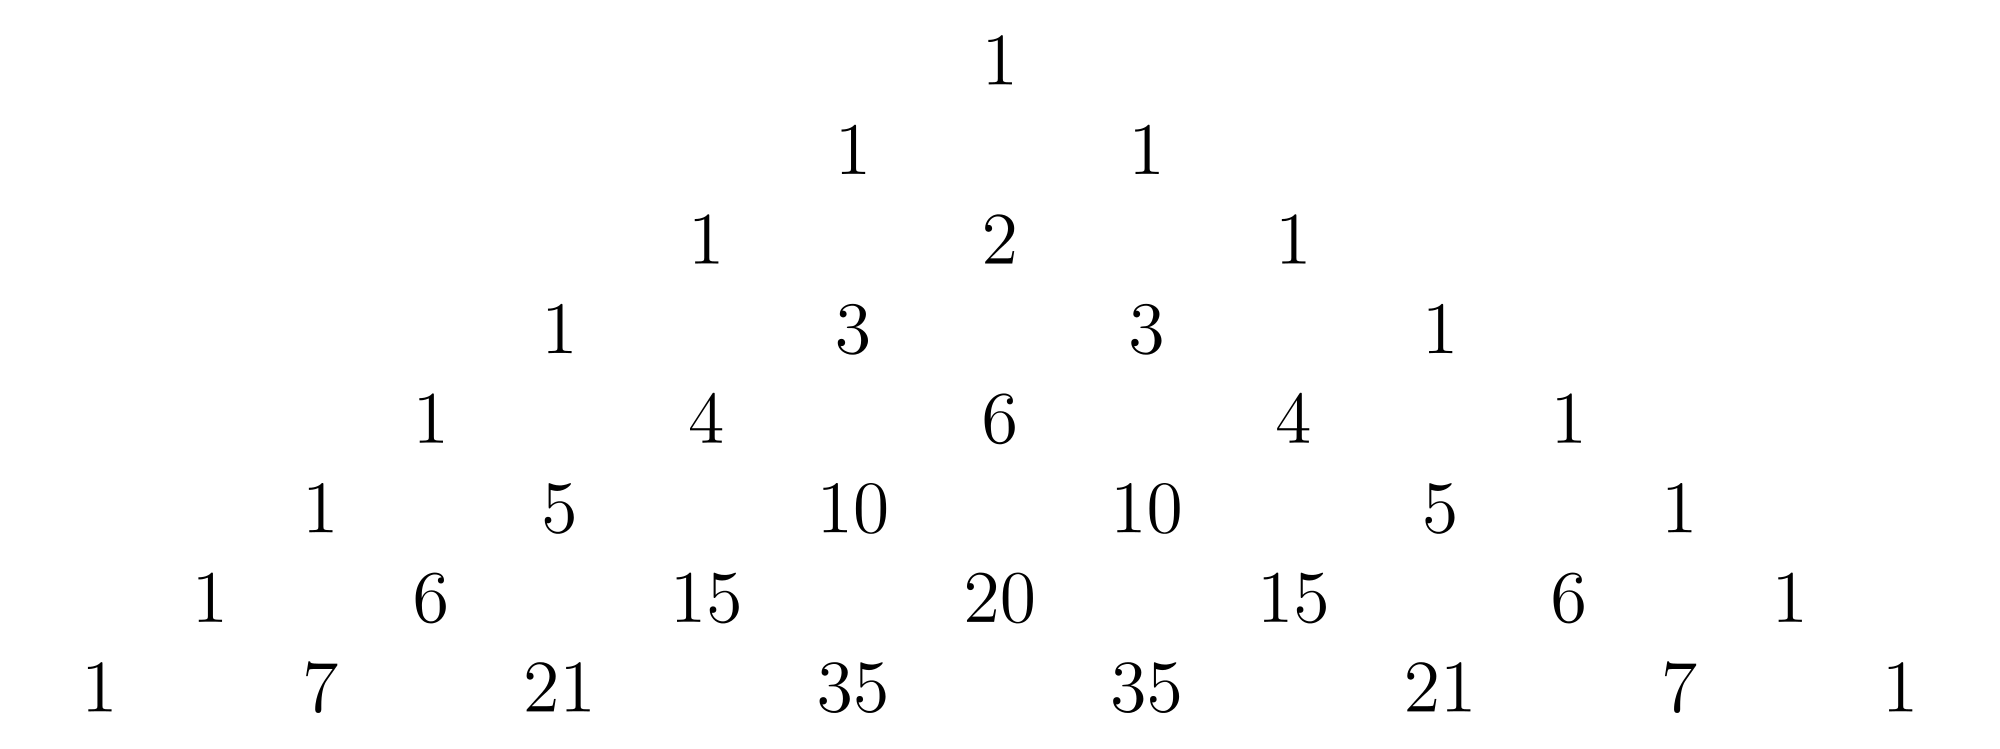
\includegraphics[scale=0.15]{binom.png}
\end{figure}
\end{frame}

\begin{frame}{Binomialkoeffizient - Implementierung}
\begin{itemize}
\item Naiv rekursiv
\begin{itemize}
\item $\rightarrow$ Viel zu langsam!
\end{itemize}
\item Vorberechnen
\begin{itemize}
\item Meist interessieren nicht alle Werte
\item $\rightarrow$ Top-Down mit Zwischenspeichern
\item Lineare Laufzeit
\end{itemize}
\item Mit nicht-rekursiver Formel
\begin{itemize}
\item Lineare Laufzeit
\end{itemize}
\end{itemize}
\end{frame}


\begin{frame} {Implementierung}
\scalebox{1.0}{
\begin{minipage}{1.0\linewidth}
\begin{algorithm} [H]
\scriptsize 
\caption{Binomialkoeffizient(n, k)}
\begin{algorithmic}
\IF {$k > n-k$}
\STATE $k \leftarrow n-k$
\ENDIF
\STATE $result \leftarrow 1$
\STATE $i \leftarrow 0$
\WHILE {$i < k$}
\STATE $result \leftarrow result \cdot \left( n - 1 \right)$
\STATE $result \leftarrow result \div \left( i + 1 \right)$
\STATE $i++$
\ENDWHILE
\STATE return $result$
\end{algorithmic}
\end{algorithm}
\end{minipage}
}
\end{frame}

\begin{frame}{Aufgabe - Der Mathetest}
\begin{itemize}
\item Gegeben: Anzahl an Faktoren
\item Gesucht: Anzahl an M"oglichkeiten, diese korrekt zu klammern
\item Beispiel:
\begin{itemize}
\item Gegeben: $\lbrace a, b, c, d \rbrace$
\item $ a \left( b \left( c d \right) \right) $ , $\left( a b \right) \left( c d \right) $ , $\left( \left( a b \right) c \right) d$ , $\left( a \left( b  c \right) \right) d $ , $ a \left( \left( b  c \right) d \right) $
\item L"osung: 5
\end{itemize}
\end{itemize}
\end{frame}

\begin{frame}{Catalan Nummern}
Definition:
\begin{align*}
Cat \left( n \right) &= \frac{1}{n+1} \binom{2n}{n} 
\end{align*}
Rekursiv:
\begin{align*}
Cat \left( 0 \right) &= 1 \\
Cat \left( n + 1 \right) &= \sum_{i=0}^n Cat \left( i \right) \cdot Cat \left( n - i \right)
\end{align*}

Also: 1, 1, 2, 5, 14, 42, 132, 429, ...
\end{frame}

\begin{frame}{Catalan Nummern}
$Cat \left( n \right)$ entspricht zum Beispiel:
\begin{itemize}
\item Anzahl verschiedener Bin"ar-B"aume mit $n$ Knoten
\item Anzahl korrekter Klammerausdruecke mit $n$ Klammerpaaren
\item Anzahl verschiedener M"oglichkeiten, $n+1$ Faktoren korrekt zu klammern
\item Anzahl M"oglichkeiten, ein konvexes $n+2$-Eck in Dreiecke aufzuteilen
\end{itemize}
\end{frame}

\begin{frame} {Implementierung}
\scalebox{1.0}{
\begin{minipage}{1.0\linewidth}
\begin{algorithm} [H]
\scriptsize 
\caption{Catalan(n)}
\begin{algorithmic}
\STATE $result = Binomialkoeffizient \left( 2 \cdot n , n \right)$
\STATE return $result \div \left(n + 1 \right)$
\end{algorithmic}
\end{algorithm}
\end{minipage}
}
\end{frame}

\begin{frame}{Catalan Nummern - Implementierung}
\begin{itemize}
\item Naiv rekursiv
\begin{itemize}
\item $\rightarrow$ Viel zu langsam! 
\end{itemize}
\item Rekursiv mit DP
\begin{itemize}
\item $\rightarrow$ Immernoch quadratische Laufzeit!
\end{itemize}
\item Mit Binomialkoeffizient
\begin{itemize}
\item $\rightarrow$ Lineare Laufzeit!
\end{itemize}
\end{itemize}
\end{frame}




\section{Spieltheorie}
\begin{frame}{Spieltheorie allgemein}
\begin{itemize}
\item Formalisierung und Darstellung von Spielen
\item Versuch, Spielausgang zu berechnen
\end{itemize}
Dabei muss gelten:
\begin{itemize}
\item Summe der Gewinne und Verluste aller Spieler betr"agt 0 (Nullsummenspiel)
\item Meistens ein Gewinner (+1) und ein Verlierer (-1)
\item Spiel ist ohne Zufall
\item Alle spielen perfekt
\end{itemize}
\end{frame}

\begin{frame}{Beispielspiel}
\begin{itemize}
\begin{block}{simples Beispielspiel}
Alice und Bob haben sechs M"unzen in der Mitte liegen und nehmen abwechselnd je eine bis drei davon. Wer die letzte M"unze nimmt, gewinnt.
\end{block}
\item Spielbaum benutzen
\end{itemize}
\end{frame}

\begin{frame}{Erstellen eines Spielbaumes}
Schritt 1:
\begin{itemize}
\item Knoten: aktueller Spieler und Spielsituation
\item Kanten: legale Spielz"uge
\item Wurzel: Spielsituation beim Start
\end{itemize}
\pause
Schritt 2:
\begin{itemize}
\item An Bl"atter des Baumes Ergebnis schreiben
\item Von unten nach oben Ergebnis berechnen
\end{itemize}
\end{frame}

\begin{frame}{Erstellen eines Spielbaumes}
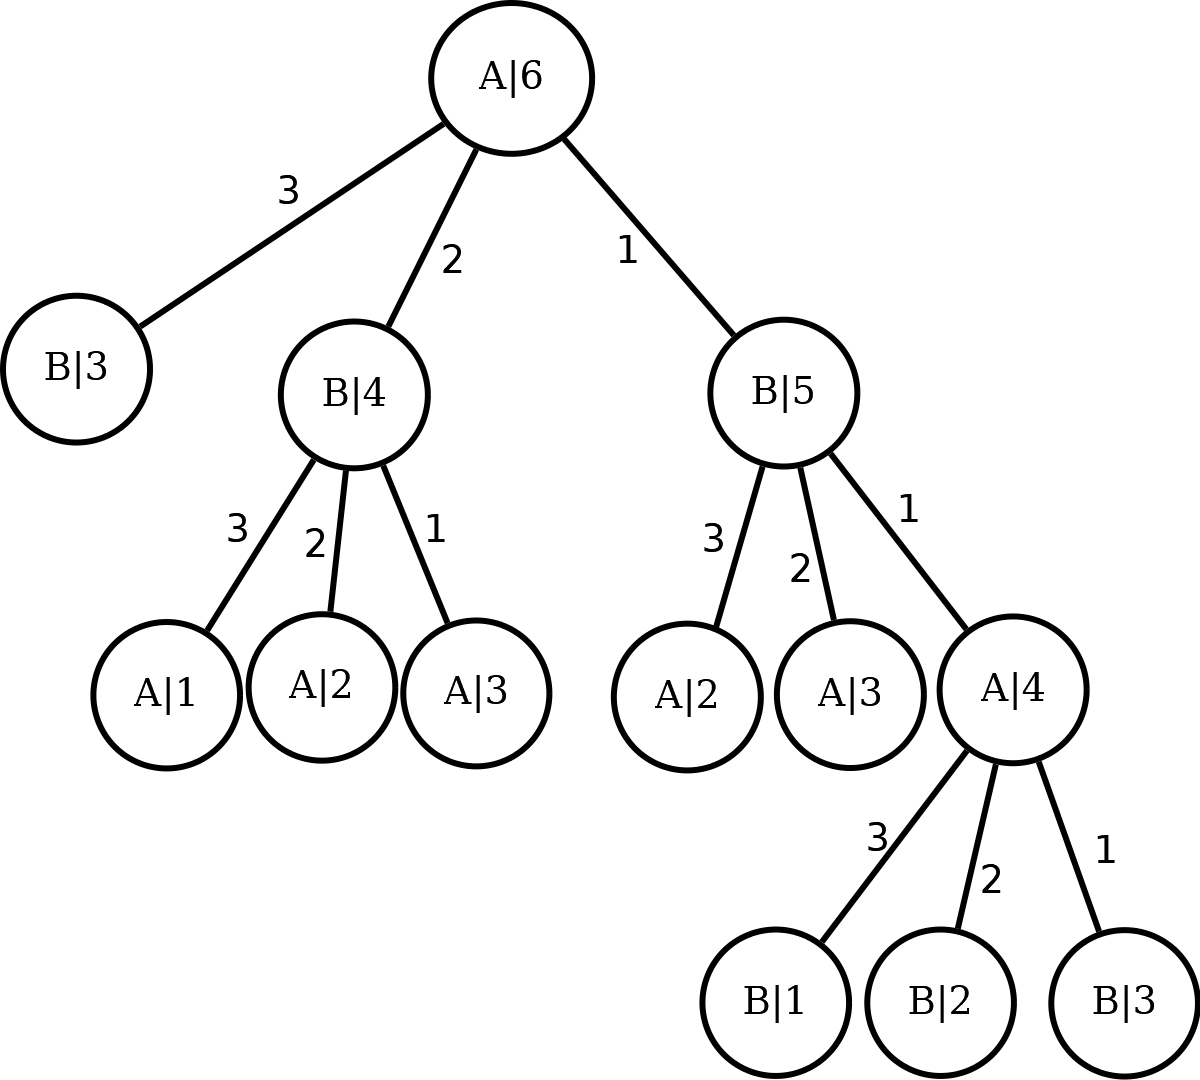
\includegraphics[scale=0.55]{baum0.png}
\end{frame}

\begin{frame}{Erstellen eines Spielbaumes}
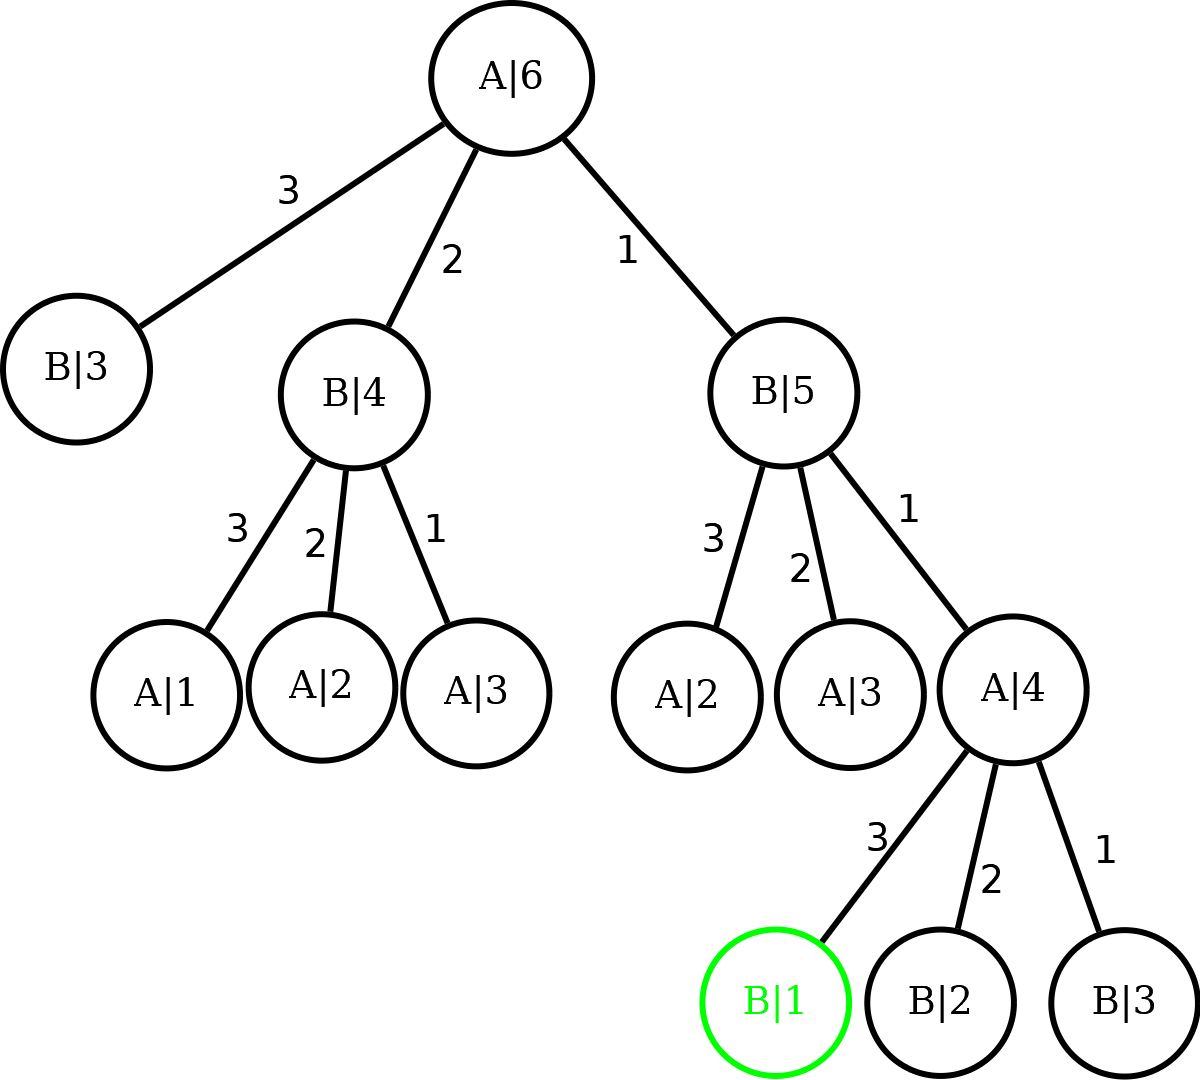
\includegraphics[scale=0.55]{baum1.png}
\end{frame}

\begin{frame}{Erstellen eines Spielbaumes}
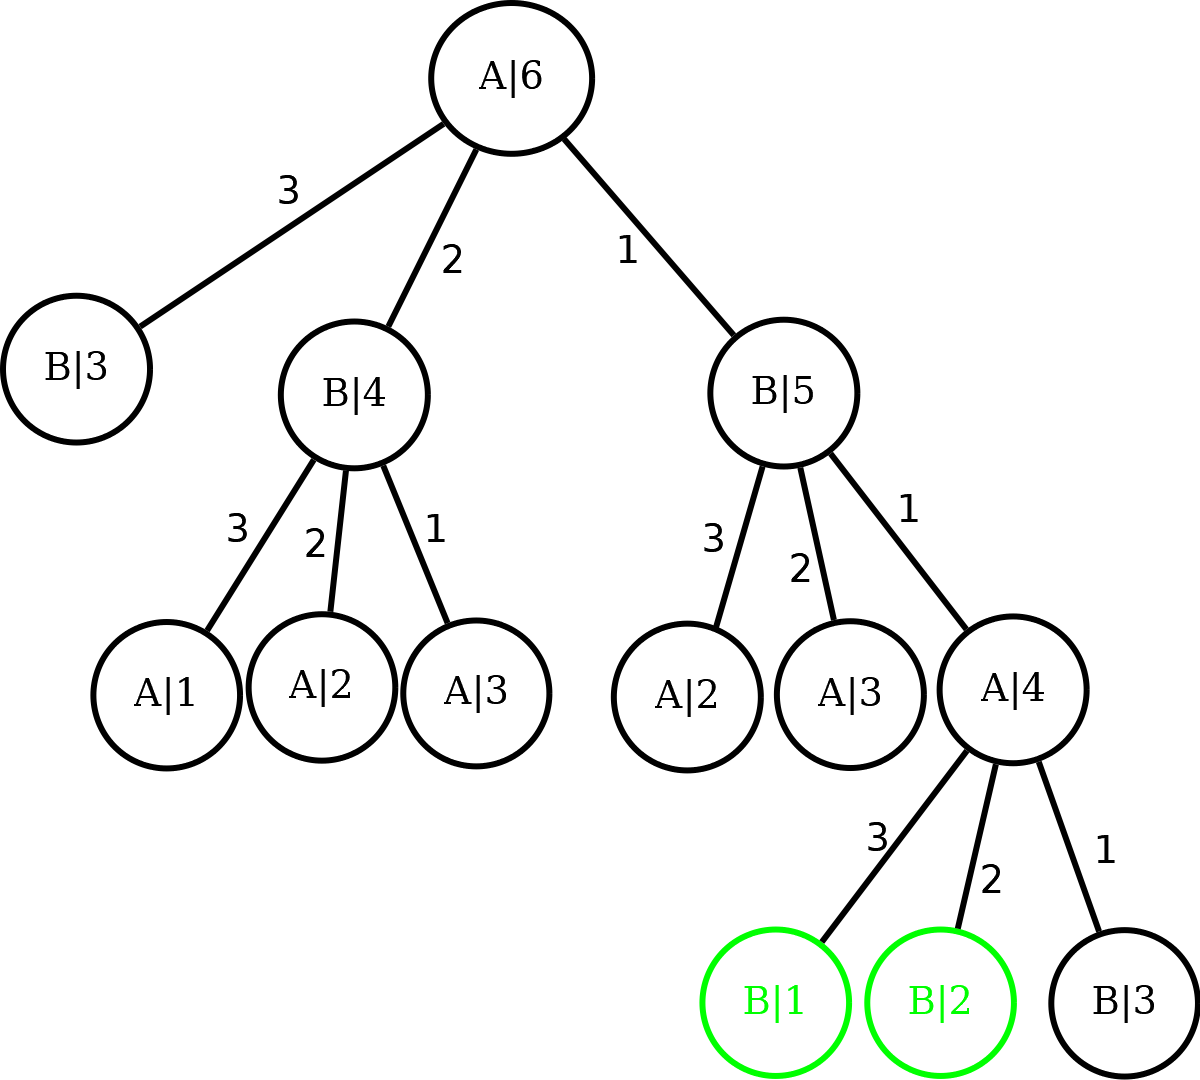
\includegraphics[scale=0.55]{baum2.png}
\end{frame}

\begin{frame}{Erstellen eines Spielbaumes}
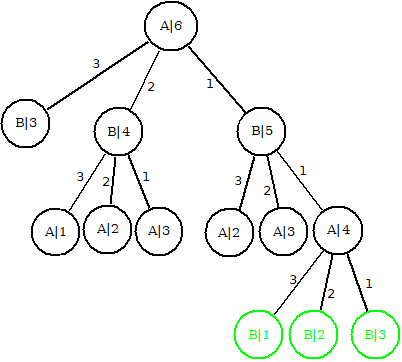
\includegraphics[scale=0.55]{baum3.png}
\end{frame}

\begin{frame}{Erstellen eines Spielbaumes}
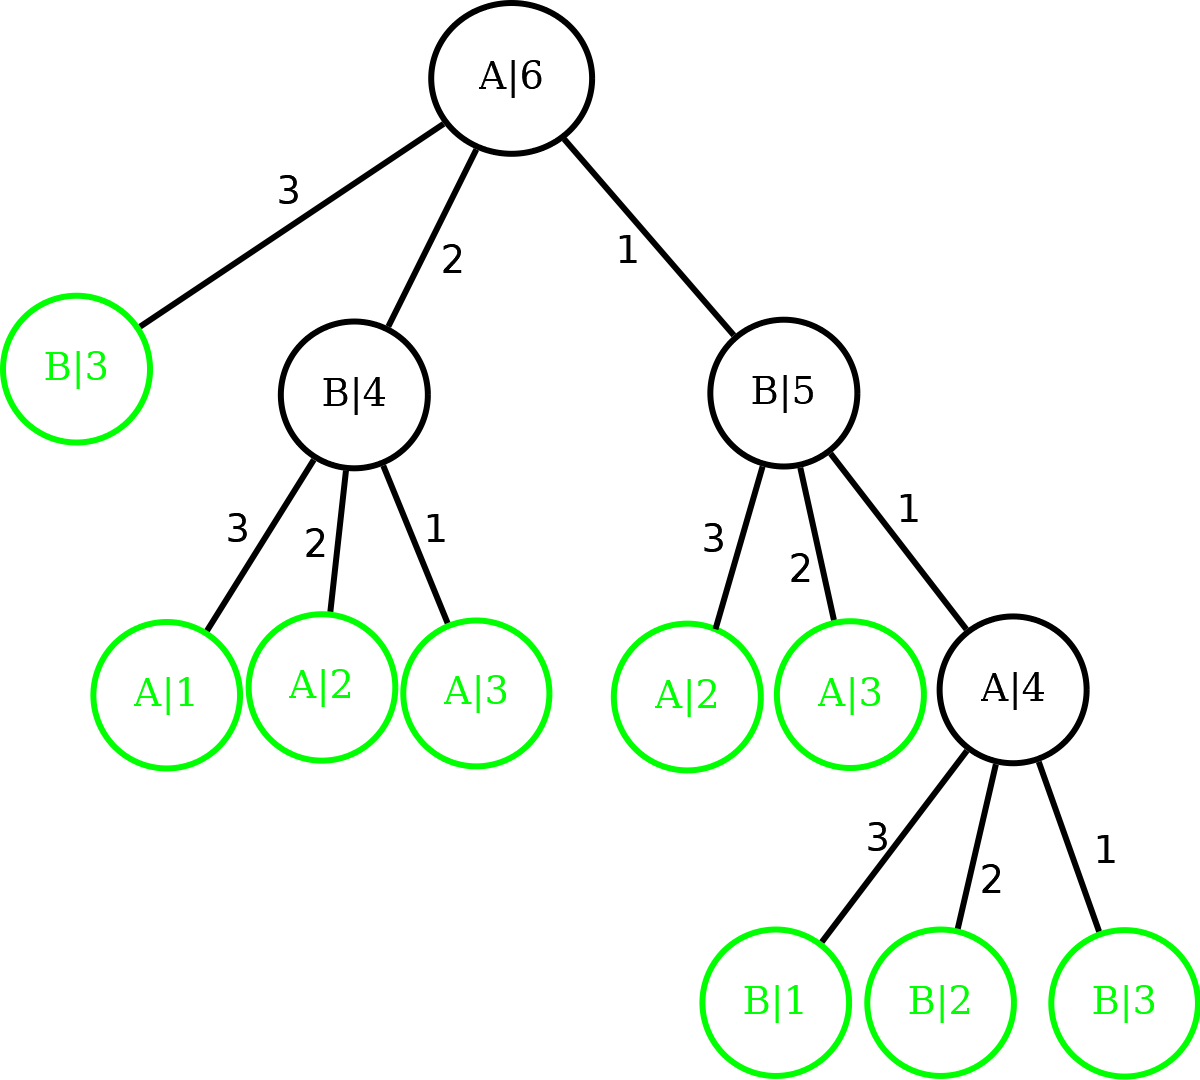
\includegraphics[scale=0.55]{baum4.png}
\end{frame}

\begin{frame}{Erstellen eines Spielbaumes}
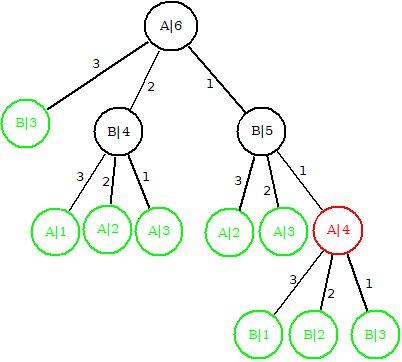
\includegraphics[scale=0.55]{baum5.png}
\end{frame}

\begin{frame}{Erstellen eines Spielbaumes}
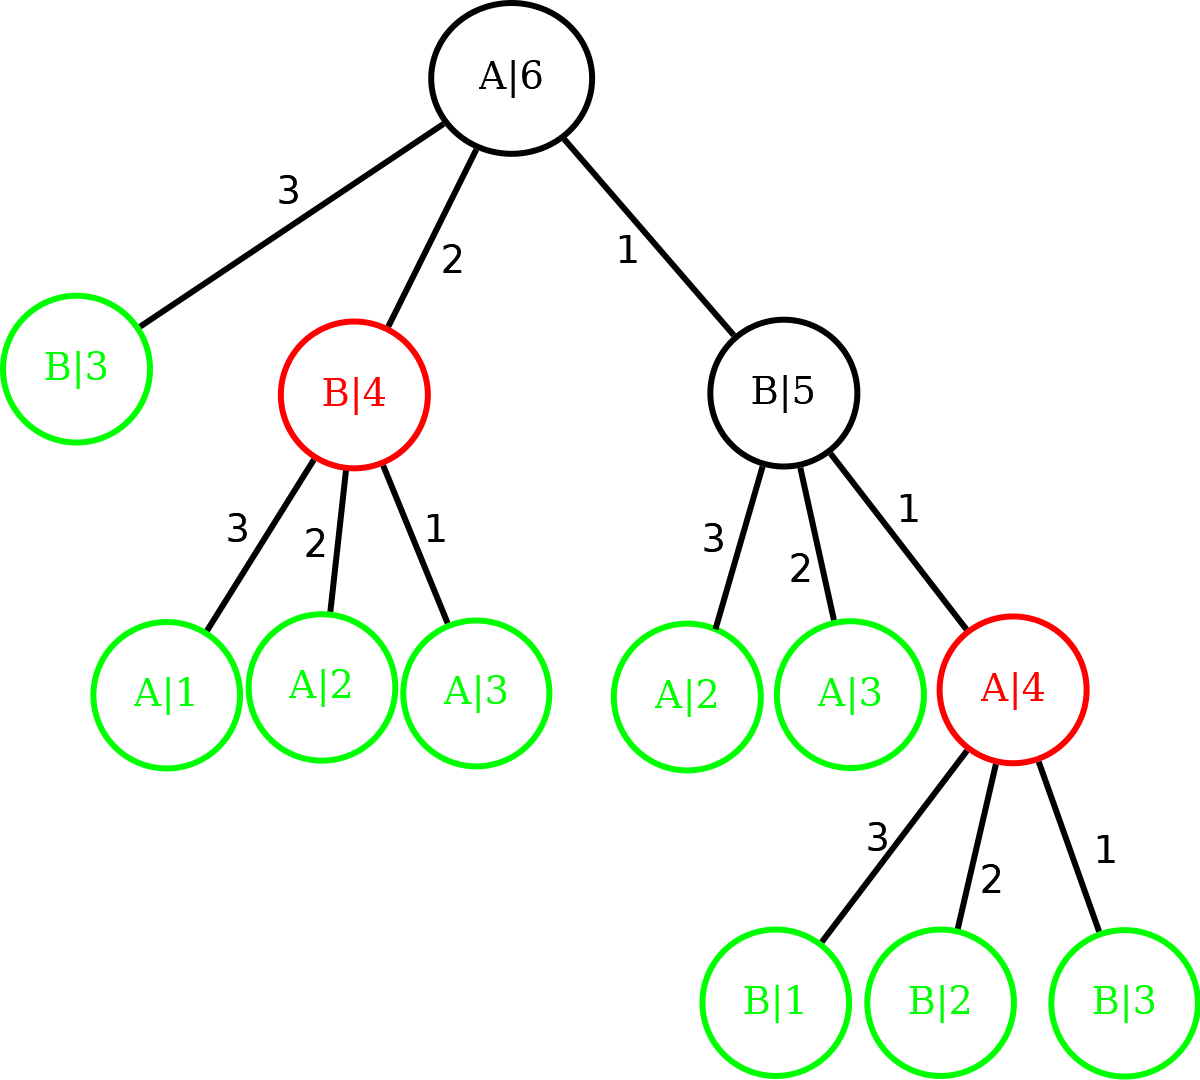
\includegraphics[scale=0.55]{baum6.png}
\end{frame}

\begin{frame}{Erstellen eines Spielbaumes}
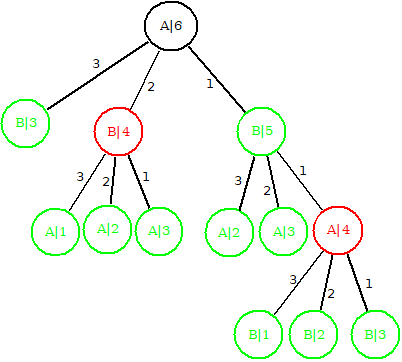
\includegraphics[scale=0.55]{baum7.png}
\end{frame}

\begin{frame}{Erstellen eines Spielbaumes}
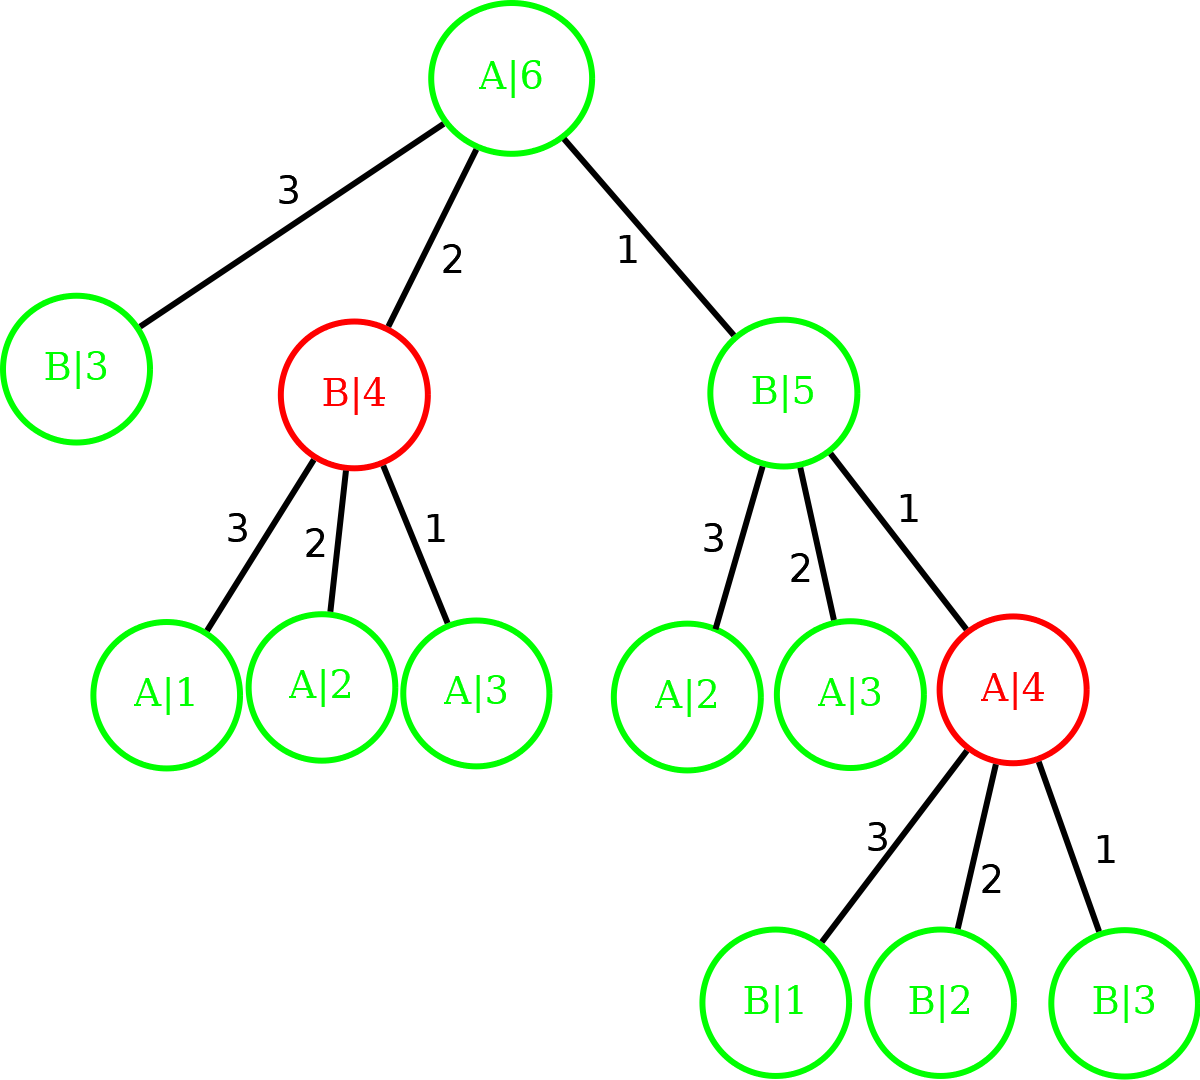
\includegraphics[scale=0.55]{baum8.png}
\end{frame}


\begin{frame}{Min-Max-Strategie}
\begin{itemize}
\item Min-Max-Strategie: Gewinn mit gr"o"stem Unterschied
\begin{equation}
   minmax(k) =
   \begin{cases}
     k.Bewertung & \text{f"ur k Blatt-Knoten} \\
     - min\left\{minmax(k') | k' Kindknoten\right\} & \text{sonst} \\
   \end{cases}
\end{equation}
\end{itemize}
\end{frame}

\begin{frame}{Andere Berechnungsm"oglichkeit}
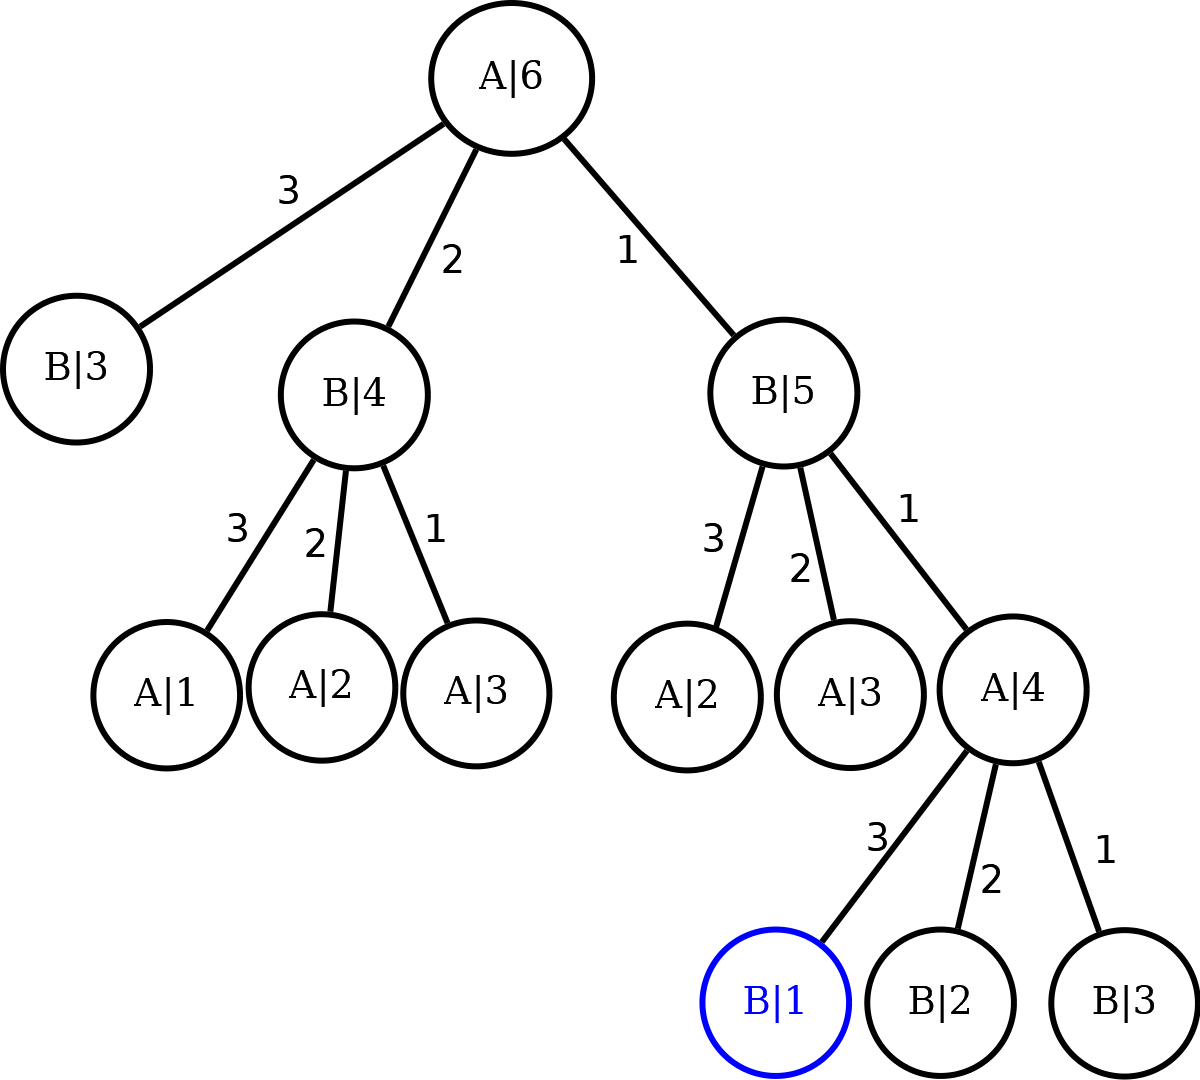
\includegraphics[scale=0.55]{baum10.png}
\end{frame}

\begin{frame}{Andere Berechnungsm"oglichkeit}
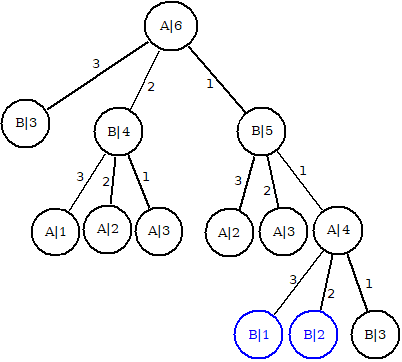
\includegraphics[scale=0.55]{baum11.png}
\end{frame}

\begin{frame}{Andere Berechnungsm"oglichkeit}
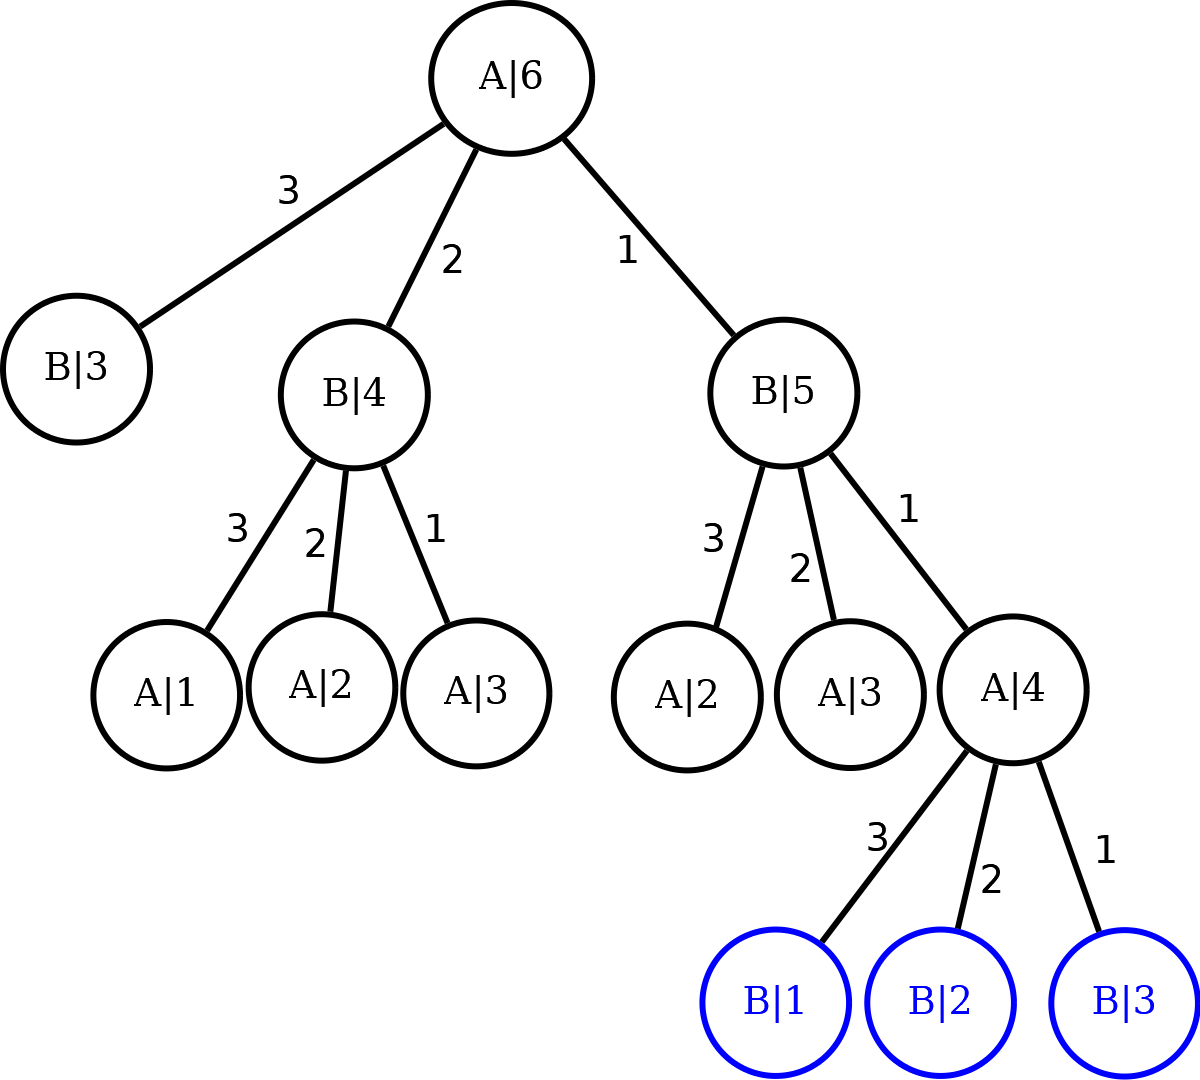
\includegraphics[scale=0.55]{baum12.png}
\end{frame}

\begin{frame}{Andere Berechnungsm"oglichkeit}
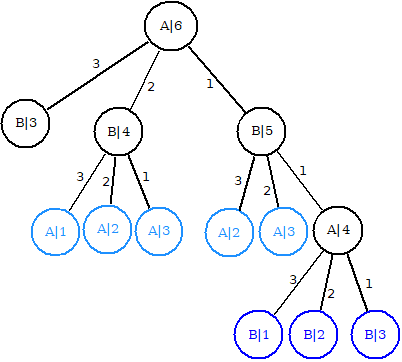
\includegraphics[scale=0.55]{baum13.png}
\end{frame}

\begin{frame}{Andere Berechnungsm"oglichkeit}
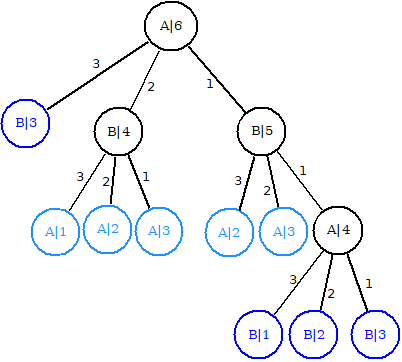
\includegraphics[scale=0.55]{baum14.png}
\end{frame}

\begin{frame}{Andere Berechnungsm"oglichkeit}
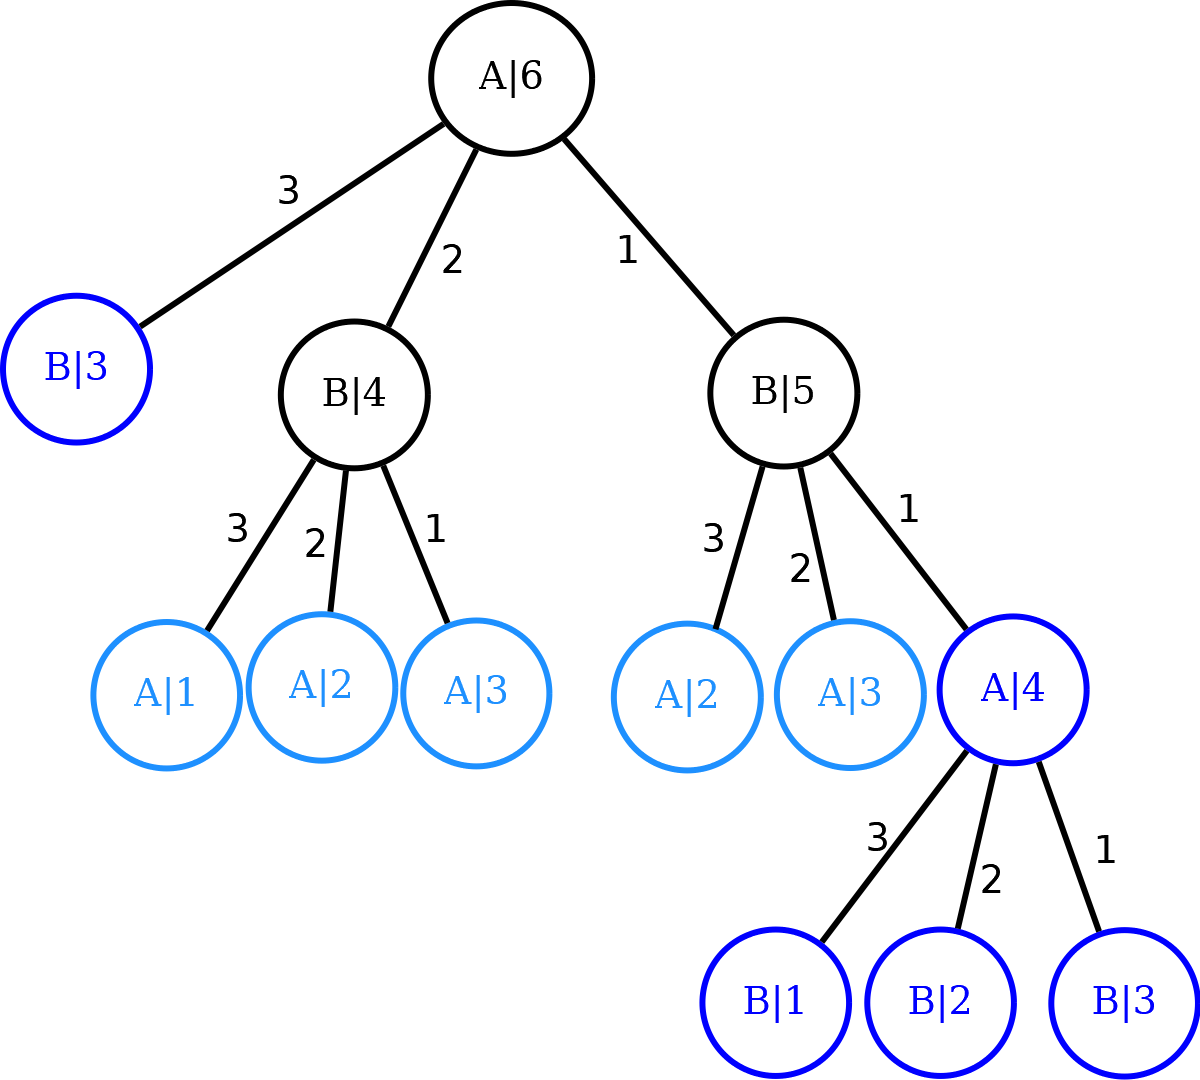
\includegraphics[scale=0.55]{baum15.png}
\end{frame}

\begin{frame}{Andere Berechnungsm"oglichkeit}
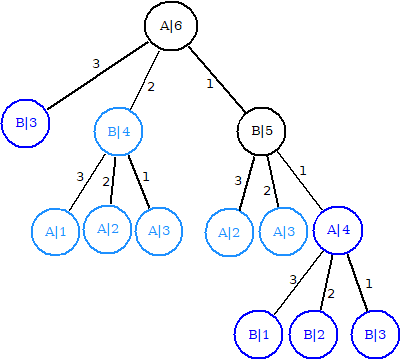
\includegraphics[scale=0.55]{baum16.png}
\end{frame}

\begin{frame}{Andere Berechnungsm"oglichkeit}
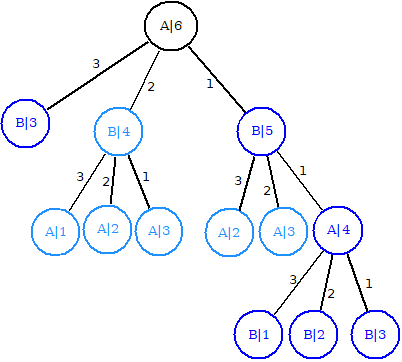
\includegraphics[scale=0.55]{baum17.png}
\end{frame}

\begin{frame}{Andere Berechnungsm"oglichkeit}
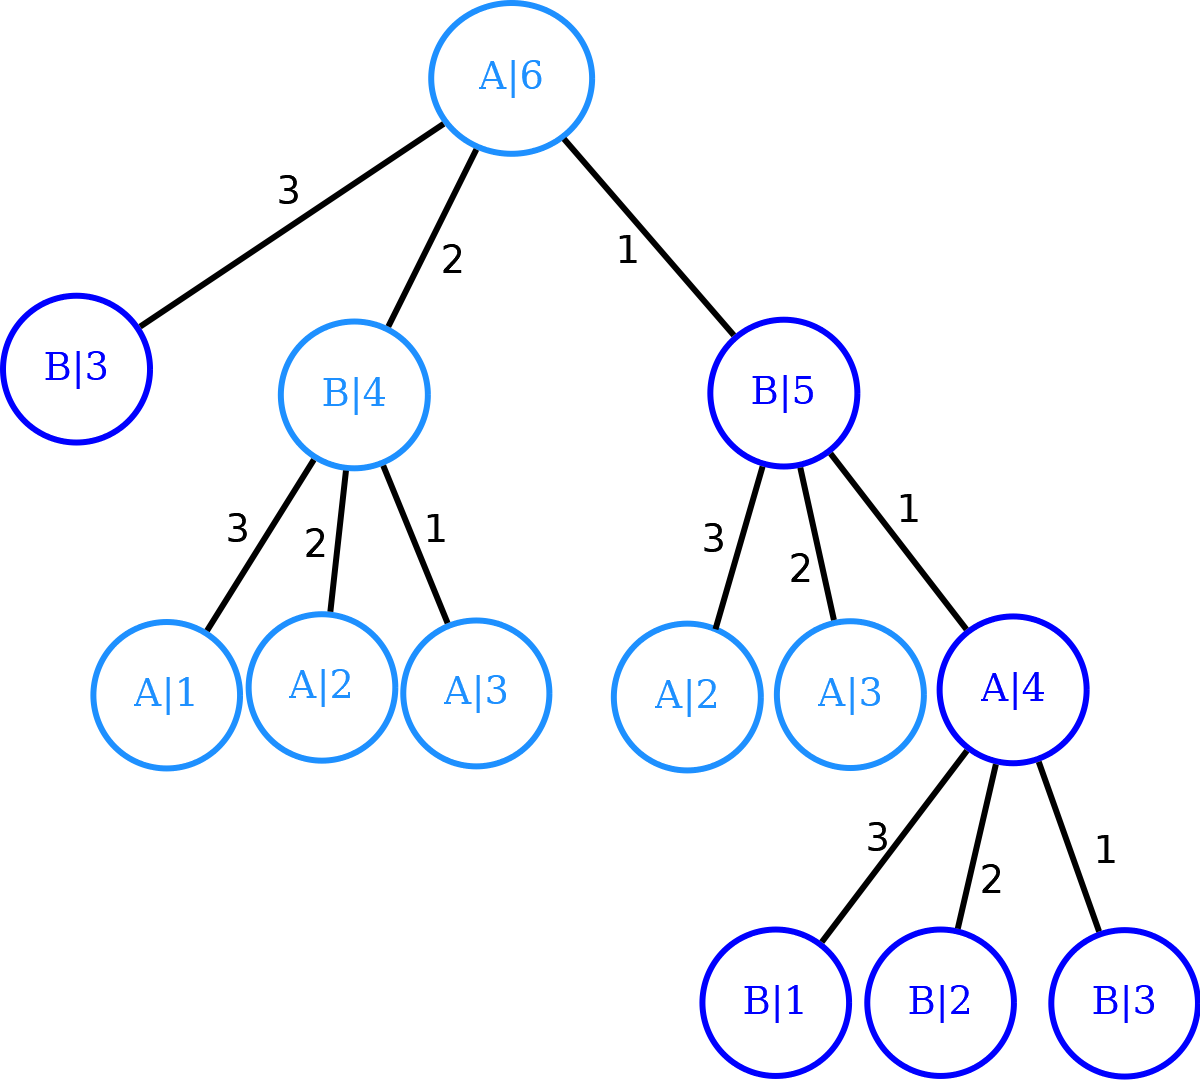
\includegraphics[scale=0.55]{baum18.png}
\end{frame}

\begin{frame}{Min-Max-Strategie}
\begin{itemize}
\item Min-Max-Strategie: Gewinn mit gr"o"stem Unterschied
\begin{equation}
   minmax(k) =
   \begin{cases}
     k.Bewertung & \text{f"ur k Blatt-Knoten} \\
     - min\left\{minmax(k') | k' Kindknoten\right\} & \text{sonst} \\
   \end{cases}
\end{equation}
\item Andere M"oglichkeit der Berechnung:
\begin{equation}
   minmax(s,k) =
   \begin{cases}
     k.Bewertung & \text{f"ur k Blatt-Knoten} \\
     min\left\{minmax(k') | k' Kindknoten\right\} & \text{falls s = A} \\
     max\left\{minmax(k') | k' Kindknoten\right\} & \text{falls s = B} \\
   \end{cases}
\end{equation}
\end{itemize}
\end{frame}

\begin{frame}{Implementierung}
\begin{itemize}
\item Wie gew"ohnt als Baum
\lstinputlisting[language=c++]{minmax1.cpp}
\item Spieler-IDs k"onnen weggelassen werden
\lstinputlisting[language=c++]{minmax2.cpp}
\end{itemize}
\end{frame}

\begin{frame}{Nachdenken nicht vergessen}
\begin{block}{Beispiel}
Die Spieler A und B multiplizieren x abwechselnd mit einer Zahl von 2 bis 9. Am Anfang ist x=1. Wer zuerst "uber eine Grenze n kommt, gewinnt.
\end{block}
\pause
\begin{itemize}
\item Problem: Je acht Kindknoten: Baum wird zu gro"s
\item L"osung: Optimale Strategie anhand kleiner B"aume herleiten
\item Im Beispiel: A nimmt immer 2, B immer 9 als Faktor
\end{itemize}
\pause
\begin{block}{Fazit}
Falls m"oglich, anhand kleiner Teilb"aume Regel herleiten, statt direkt anzufangen, zu implementieren.
\end{block}
\end{frame}

\begin{frame}{Nim-Spiel}
\begin{itemize}
\item Mehrere Haufen mit Objekten
\item Zwei Spieler nehmen abwechselnd von einem Haufen
\item Wer das letzte Objekt nimmt, gewinnt
\item F"ur wenigei Haufen mit Spielbaum modellierbar
\item F"ur viele Haufen eigene Optimalstrategie n"otig
\end{itemize}
\end{frame}

\begin{frame}{Nim-Spiel: Optimalstrategie}
\begin{itemize}
\item Nim-Zahl: Anzahl Objekte in Haufen bin"ar mit XOR verkn"upfen
\item Gewinnstrategie: In jedem Zug die Nim-Zahl auf 0 bringen
\begin{block}{Beispiel}
5 Haufen mit 6, 3, 5, 2 und 7 Elemente \\
Bin"ar: 110\textsubscript{2}, 011\textsubscript{2}, 101\textsubscript{2}, 010\textsubscript{2} und 111\textsubscript{2} Elemente\\
Dann: 110\textsubscript{2} XOR 011\textsubscript{2} XOR 101\textsubscript{2} XOR 010\textsubscript{2} XOR 111\textsubscript{2} = 101\textsubscript{2} \\
Der Spieler am Zug hat also die M"oglichkeit, die Nim-Zahl auf 0 zu bringen (z. B. indem er vom letzten Stapel 5 Elemente entfernt), und hat somit eine Gewinnstrategie.
\end{block}
\end{itemize}
\end{frame}

\begin{frame}{Grundy-Zahlen}
\begin{itemize}
\item Theorem von Sprague-Grundy: Jedes neutrale Spiel "aquivalent zu Standard-Nim-Spiel
\item Grundy-Zahlen: kleinste Zahl, die nicht Grundy-Zahl von Nachfolgerstellung ist
\item Nim-Zahlen entsprechen Grundy-Zahlen
\item Gewinnstrategie: Grundy-Zahl in jedem Zug auf 0 bringen
\end{itemize}
\end{frame}

\begin{frame}{Grundy-Zahlen - Beispiel}
\begin{block}{Beispiel}
Es gibt drei Haufen mit einem, zwei und drei Elementen. Berechne die Grundy-Zahl dieser Situation
\end{block}
Es gibt sechs m"ogliche Nachfolgerzust"ande:
\begin{itemize}
\pause
\item 0, 2 und 3 Elemente: 000\textsubscript{2} XOR 010\textsubscript{2} XOR 011\textsubscript{2} = 001\textsubscript{2} = 1
\pause
\item 1, 1 und 3 Elemente: 001\textsubscript{2} XOR 001\textsubscript{2} XOR 011\textsubscript{2} = 011\textsubscript{2} = 3
\pause
\item 1, 0 und 3 Elemente: 001\textsubscript{2} XOR 000\textsubscript{2} XOR 011\textsubscript{2} = 010\textsubscript{2} = 2
\pause
\item 1, 2 und 0 Elemente: 001\textsubscript{2} XOR 010\textsubscript{2} XOR 000\textsubscript{2} = 011\textsubscript{2} = 3
\pause
\item 1, 2 und 1 Elemente: 001\textsubscript{2} XOR 010\textsubscript{2} XOR 001\textsubscript{2} = 010\textsubscript{2} = 2
\pause
\item 1, 2 und 2 Elemente: 001\textsubscript{2} XOR 010\textsubscript{2} XOR 010\textsubscript{2} = 010\textsubscript{2} = 2
\pause
\item Kleinste nicht vorkommende Zahl ist 0, also keine Gewinnstrategie
\end{itemize}
\end{frame}

\begin{frame}{ICPC-Aufgabe}
\end{frame}


\end{document}
